\title{Plan de Trabajo}
\author{
        Beñat Agirre Arruabarrena \\
        b.agirre@alumnos.upm.es \\
}
\date{\today}

\documentclass[11pt]{article}
\usepackage[spanish]{babel}
\usepackage{graphicx}
\graphicspath{ {./images/} }
\usepackage{pdfpages}
\usepackage{fullpage}

\begin{document}
\maketitle
\tableofcontents
\newpage

%%%%%%%%%%%%%%%%%%%%%%%%%%%%%%%%%%%%%%%%%%%%%%%%%%%%%%%%%%%%%%%%%%%%%%%%%%%%%%%%%%%%%%%%%%%%%%%%%%%%%%%%
\section{Descripción general del trabajo}
El objetivo principal del trabajo es introducir soporte al formato GeoPackage en herramientas de Linked Data
Geográfico desarrolladas por el Grupo de Ingeniería Ontológica.
En el Grupo de Ingeniería Ontológica se ha venido tradicionalmente trabajando con el Instituto Geográfico Nacional para la exportación de algunos de sus datos geográficos a formato Linked Data. Un ejemplo se puede encontrar en https://datos.ign.es/

Recientemente, el Open Geospatial Consortium ha publicado el formato GeoPackage, que tiene el objetivo de convertirse en un estándar para la representación de datos geográficos. El objetivo de este trabajo es el de dar soporte GeoPackage para las herramientas normalmente utilizadas para este tipo de tareas.

%%%%%%%%%%%%%%%%%%%%%%%%%%%%%%%%%%%%%%%%%%%%%%%%%%%%%%%%%%%%%%%%%%%%%%%%%%%%%%%%%%%%%%%%%%%%%%%%%%%%%%%%
\subsection{Objetivos}
\begin{itemize}
    \item Dar soporte GeoPackage a la herramienta Map4RDF
    \item Dar soporte GeoPackage a la herramienta GeoKettle y su plugin para transformar a RDF
    \item Realizar un procesado completo de todos los datos del IGN para generar este tipo de formato.
\end{itemize}

%%%%%%%%%%%%%%%%%%%%%%%%%%%%%%%%%%%%%%%%%%%%%%%%%%%%%%%%%%%%%%%%%%%%%%%%%%%%%%%%%%%%%%%%%%%%%%%%%%%%%%%%
\section{Lista de tareas}
\begin{itemize}
    \item Análisis del formato GeoPackage y herramientas asociadas: 20\%
    \item Diseño de soluciones: 20\%
    \item Implementación de soluciones: 40\%
    \item Evaluación: 10\%
    \item Documentación: 10\%
\end{itemize}

\section{Diagrama de Gantt}
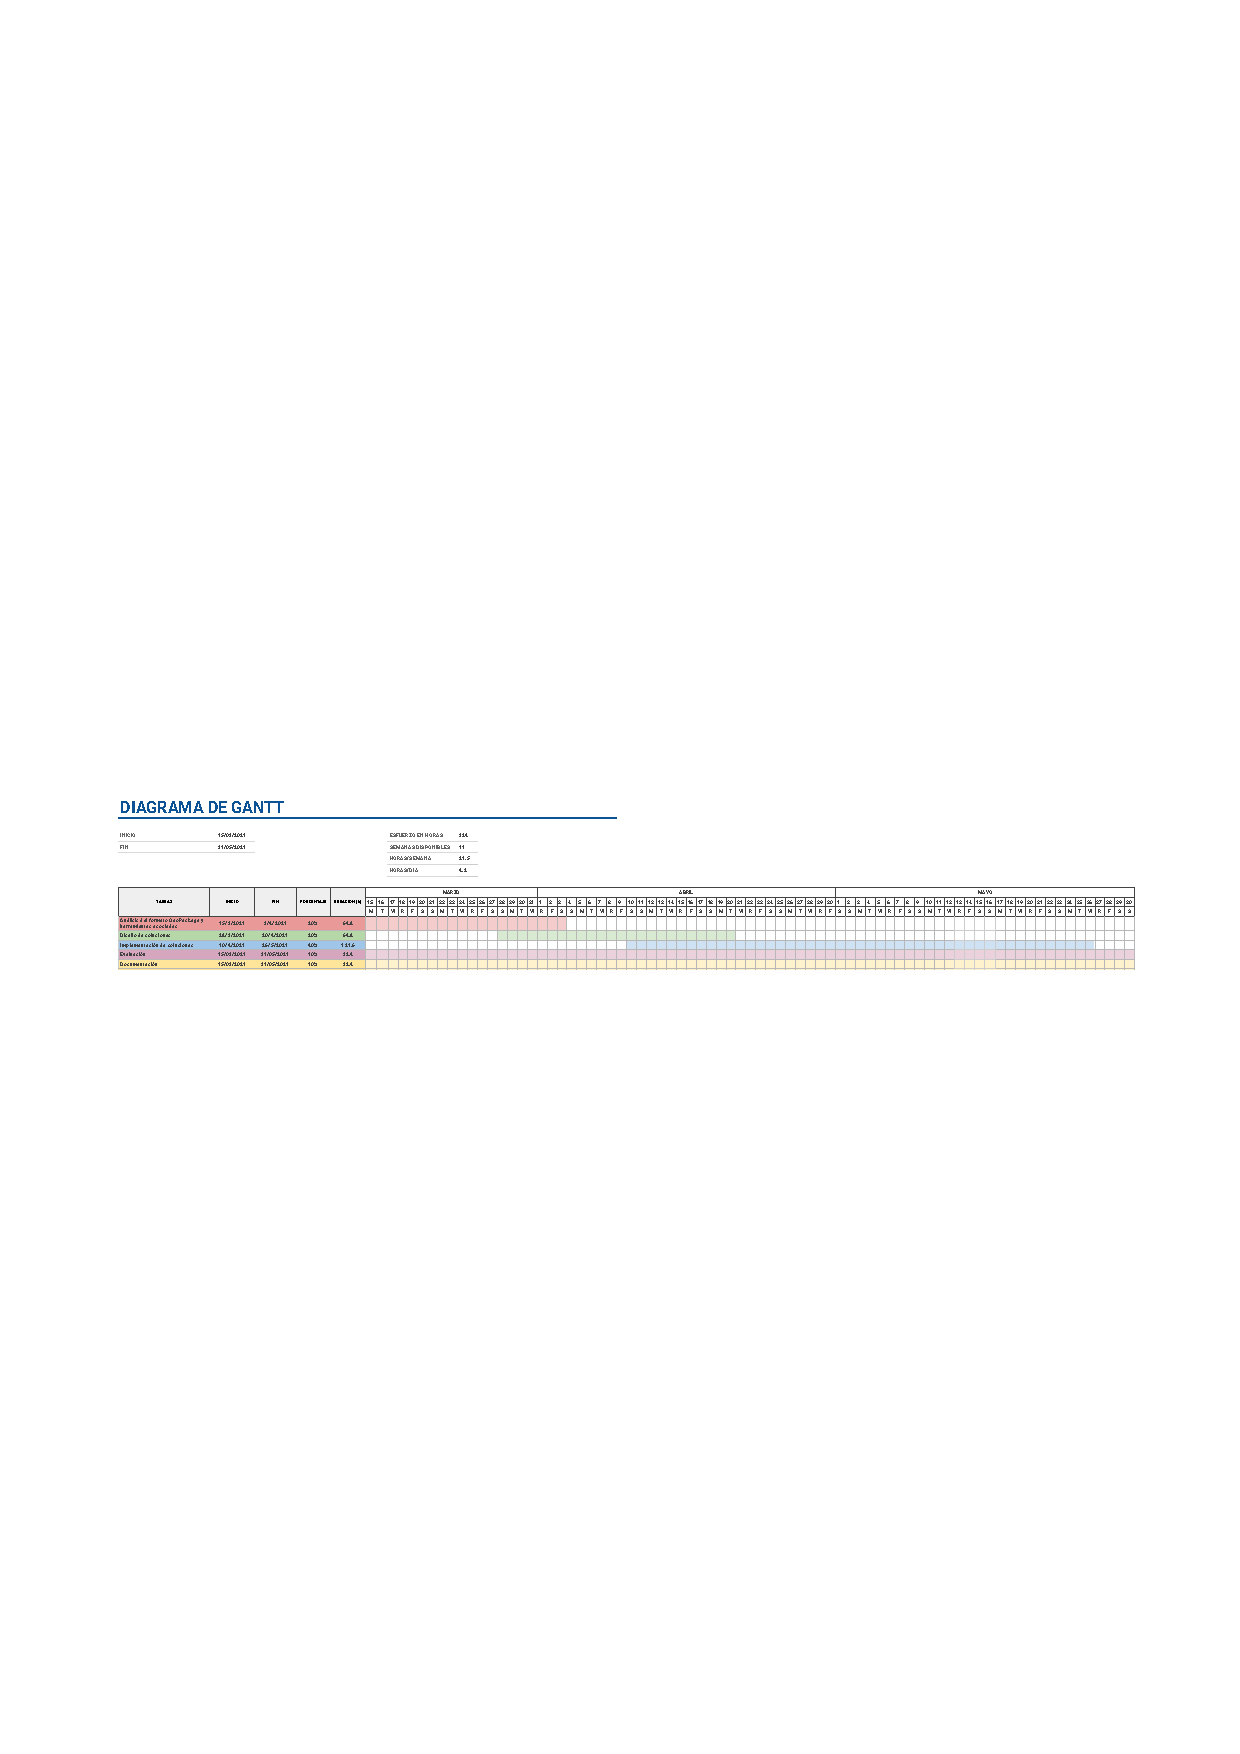
\includepdf[pages=-]{Gantt.pdf}


%%%%%%%%%%%%%%%%%%%%%%%%%%%%%%%%%%%%%%%%%%%%%%%%%%%%%%%%%%%%%%%%%%%%%%%%%%%%%%%%%%%%%%%%%%%%%%%%%%%%%%%%
\section{Copia de la propuesta de trabajo escrito por el tutor}
\begin{figure}[h]
    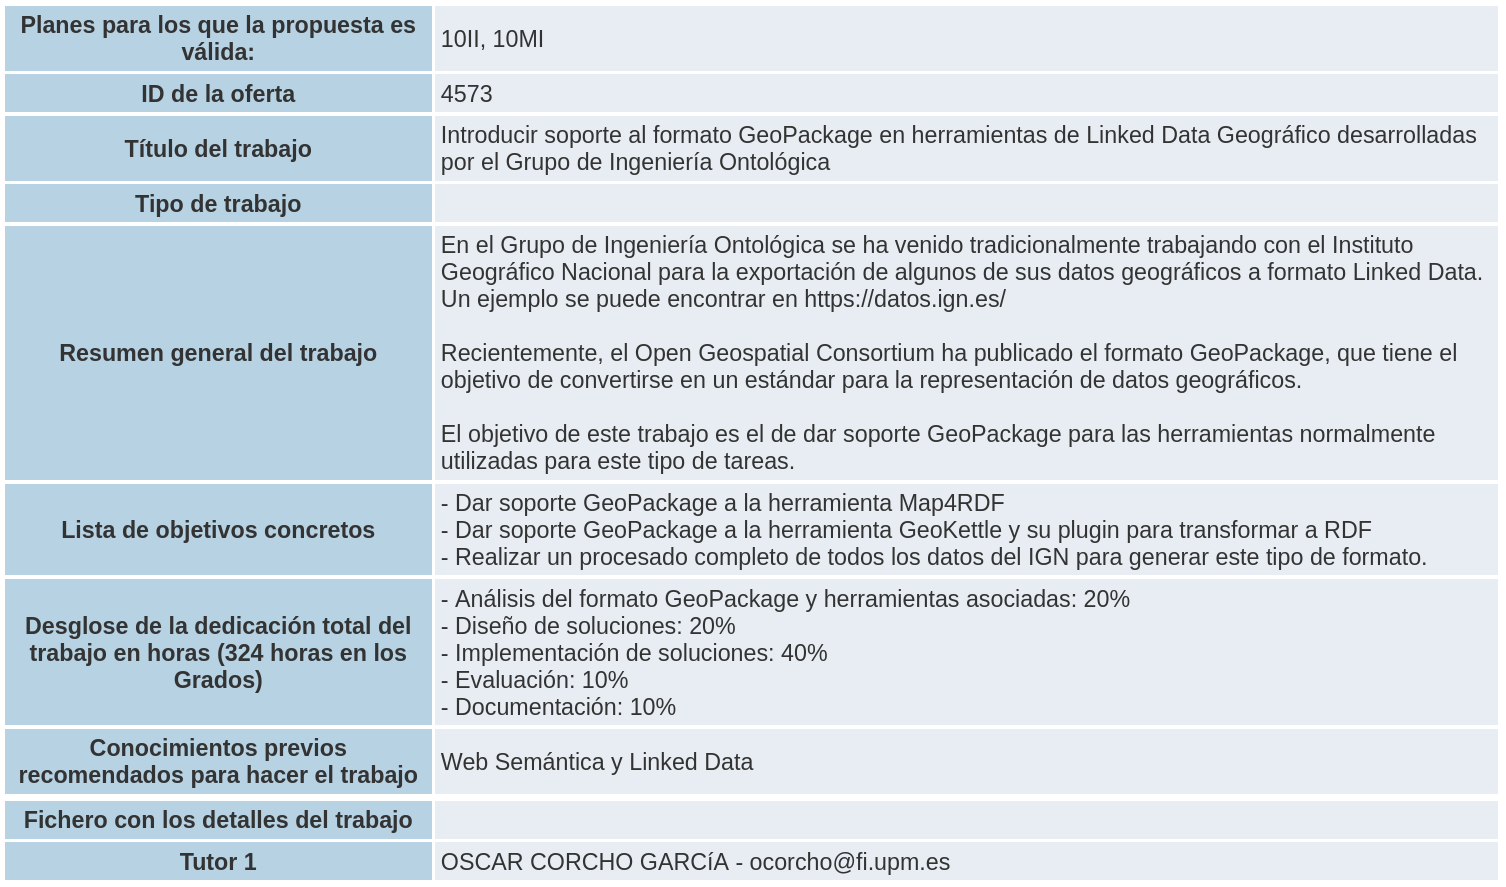
\includegraphics[width=\textwidth]{./copia.png}
    \centering
    \caption{Propuesta de trabajo}
    \label{fig:propuesta}
\end{figure}

%%%%%%%%%%%%%%%%%%%%%%%%%%%%%%%%%%%%%%%%%%%%%%%%%%%%%%%%%%%%%%%%%%%%%%%%%%%%%%%%%%%%%%%%%%%%%%%%%%%%%%%%

\end{document}
